\chapter{Estudo de Casos}
\label{cap5}
Este capítulo apresenta um estudo de caso do Cloudooo e sua implantação no ERP5. O estudo de caso foi idealizado para mostrar a instalação, configuração e uso do Cloudooo no ERP5. Além disso, foi realizado uma comparação entre o Cloudooo e o OOOD.

\section{Ambiente de desenvolvimento}
Para desenvolvimento foi utilizado uma máquina com processador AMD Turion X2 1.6, 2 GB de RAM e 160 GB de HD. O sistema operacional utilizado foi o Mandriva na versão 2010.0, o mesmo que o ERP5 é desenvolvido.

Como pré-requisito de instalação foi necessário ter instalado no sistema operacional o Xvfb e o Python na versão 2.6, pois o OpenOffice.org é instalado junto com a aplicação.

\section{Instalação do Cloudooo}
Para instalação de toda estrutura, é utilizado o Buildout. Este mecanismo de instalação criará um ambiente com todos os pré-requisitos instalados dentro da própria estrutura do Buildout, exceto bibliotecas e aplicativos do sistema operacional. No sistema operacional é necessário que tenha instalado o Xvfb e um Python na versão 2.6 e o pacote \textit{Subversion}.

O procedimento de instalação, após a instalação de todas dependências do sistema operacional, foi fazer download através do repositório SVN \url{https://svn.erp5.org/repos/experimental/oood.buildout}. Este Buildout, foi programado para fazer download do OOOD, que se encontra no repositório SVN \url{http://svn.erp5.org/repos/experimental/oood}. Após isto, acessou-se a pasta que foi criada em seu sistema operacional e executar o arquivo bootstrap.py dentro da pasta bootstrap com o Python 2.6. Com a execução do bootstrap.py, toda estrutura daquela pasta estará ligada diretamente ao python que foi executado. Para ser feita a instalação de todos pacotes necessários e o OpenOffice.org é preciso executar o comando ``bin/buildout'' dentro da mesma pasta.

Na execução deste último comando, além de todas bibliotecas, foi instalado também um OpenOffice.org, versão 3.2, dentro da mesma estrutura. Esta solução foi criada para facilitar a instalação, além de unificar e organizar toda estrutura em um só lugar.

\section{Todos os passos de uma resposta ao cliente}

Para um cliente se conectar ao serviço OOOD, a biblioteca utilizada para comunicação entre o cliente e o servidor é a \textit{xmlrpclib}. A Figura \ref{fig:xmlrpclib.png} demonstra um exemplo de como se conectar ao serviço utilizando a linguagem de programação Python, realizando o envio de uma requisição para o servidor.

\begin{figure}[!ht]
\centering
\begin{center}
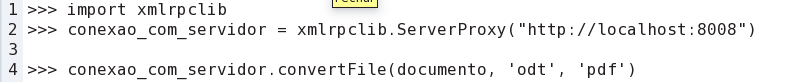
\includegraphics[scale=0.660,bb=0 0 600 50]{cliente.png}
\end{center}
\caption{Conexão do cliente com servidor.}
\label{fig:xmlrpclib.png}
\end{figure}

As etapas para conversão de um documento são:
\begin{itemize}
\item O servidor recebe os dados do cliente e estes são inseridos no objeto instanciado \textit{OOHandler};
\item Quando o \textit{OOHandler} recebe os dados, um objeto \textit{FileSystemDocument} é criado para salvar estes dados;
\item Para conversão dos dados, o \textit{OOHandler} bloqueia o objeto OpenOffice para uso, caso este esteja liberado. Caso contrário a requisição espera a liberação do objeto OpenOffice;
\item Quando a conversão do documento é finalizada, o objeto OpenOffice é desbloqueado;
\item Por fim, os dados convertidos são enviados para o cliente e a requisição é toda excluída inclusive os dados armazenados pelo \textit{FileSystemDocument};
\end{itemize}

\section{Instalação do ERP5}
Utilizando o pacote \textit{Subversion}, foi realizado \textit{download} do Buildout para instalação das dependências do ERP5. A Figura \ref{fig:erp5_software} demonstra como fazer \textit{download} do Buildout.

\begin{figure}[!ht]
\centering
\begin{center}
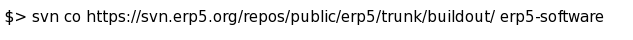
\includegraphics[scale=0.660,bb=0 30 600 20]{erp5_software.png}
\end{center}
\caption{\textit{Download} do Buildout para instalação das dependências do ERP5. Fonte: \cite{erp5_buildout}.}
\label{fig:erp5_software}
\end{figure}

Antes do \textit{download}, foi necessário aceitar um certificado para que os arquivos sejam copiados para a máquina local. Para aceitar este certificado, foi selecionado a opção ``permanente'' para que isto não seja perguntado novamente.

Com os arquivo copiados na máquina local, o próximo passo é instalar todas as dependências através de um \textit{script} que está dentro da pasta ``erp5-software'', criada pelo passo anterior. O comando de execução deste \textit{script} pode ver visto na Figura \ref{fig:dependencies}.

\begin{figure}[!ht]
\centering
\begin{center}
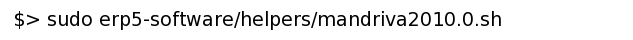
\includegraphics[scale=0.600,bb=0 30 500 20]{erp5_dependencies.png}
\end{center}
\caption{Comando para instalar dependências. Fonte: \cite{erp5_buildout}.}
\label{fig:dependencies}
\end{figure}

Devidamente instaladas todas dependências, o Buildout é executado para instalação dos \textit{softwares}, como por exemplo MySQL, Flare, OOOD. A Figura \ref{fig:make_software} demonstra como executar este comando.

\begin{figure}[!ht]
\centering
\begin{center}
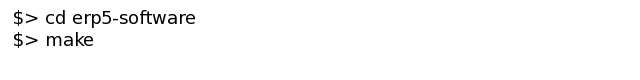
\includegraphics[scale=0.660,bb=0 40 400 65]{make_software.png}
\end{center}
\caption{Comando para instalar configurar o Buildout com as dependências instaladas no sistema operacional. Fonte: \cite{erp5_buildout}.}
\label{fig:make_software}
\end{figure}

Terminada a execução do Buildout, outra estrutura será utilizada para instalação de uma instância do ERP5. Esta separação é aconselhada, pois caso seja necessário criar uma outra instância, já exite um ambiente com todas as dependências instaladas. Então, para instalar a instância, utiliza-se novamente o Buildout, como demonstra a Figura \ref{fig:erp5_data}.

\begin{figure}[!ht]
\centering
\begin{center}
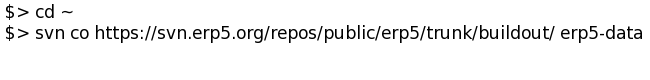
\includegraphics[scale=0.660,bb=50 50 600 70]{erp5_data.png}
\end{center}
\caption{\textit{Download} do Buildout para instalação de uma instância do ERP5. Fonte: \cite{erp5_buildout}.}
\label{fig:erp5_data}
\end{figure}

Novamente após o \textit{download} do Buildout, uma pasta será criada localmente mas com o nome de ``erp5-data''. Nesta pasta são utilizados arquivos de configurações já predefinidos para instalação e configuração da instância do ERP5. Para iniciar a configuração do Buildout foi criado um arquivo com a configuração apresentada na Figura \ref{fig:my_config}, nome ``my\_config.cfg'' e salvo dentro da pasta ``erp5-data''.

\begin{figure}[!ht]
\centering
\begin{center}
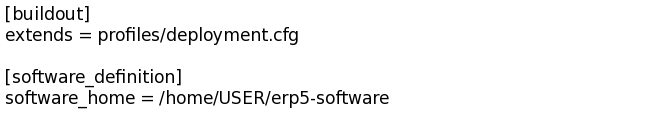
\includegraphics[scale=0.660,bb=0 50 400 120]{erp5_minha_instancia.png}
\end{center}
\caption{Arquivo de configuração ``my\_config.cfg''. Fonte: \cite{erp5_buildout}.}
\label{fig:my_config}
\end{figure}

Note que na Figura \ref{fig:my_config}, possui o nome \textit{USER} no campo ``caminho da pasta''. Este nome deve ser substituido pelo nome do usuário da máquina.

Com este arquivo de configuração, esta instância foi configurada para utilizar todas dependências instaladas no Buildout criado anteriormente. Com isso, não será necessário instalar todos \textit{softwares} novamente, pois esta instância estará utilizando todos recursos do Buildout instalado na pasta ``erp5-software''. A Figura \ref{fig:run_base_instance} apresenta os comandos para configuração desta instância.

\begin{figure}[!ht]
\centering
\begin{center}
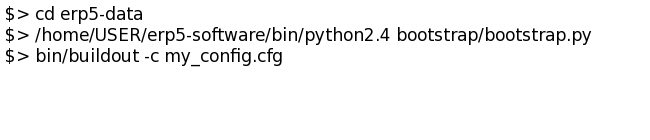
\includegraphics[scale=0.660,bb=0 90 610 120]{run_minha_instancia.png}
\end{center}
\caption{Comandos que configuram as dependências no novo Buildout. Fonte: \cite{erp5_buildout}.}
\label{fig:run_base_instance}
\end{figure}

Após isto, a instância já está configurada com os \textit{softwares}, que serão utilizados pelo ERP5, como por exemplo o OOOD. Com o comando apresentado na Figura \ref{fig:supervisor}, todos estes aplicativos são iniciados.

\begin{figure}[!ht]
\centering
\begin{center}
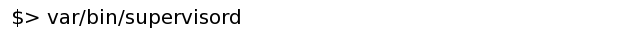
\includegraphics[scale=0.660,bb=0 30 410 5]{erp5_supervidor.png}
\end{center}
\caption{Comando para iniciar todos aplicativos. Fonte: \cite{erp5_buildout}.}
\label{fig:supervisor}
\end{figure}

Com todas as dependências iniciadas, como por exemplo MySQL e Cloudooo, o próximo passo é a criação da configuração com nome de ``development.cfg'' para criação da instância do ERP5 instalada, desmonstrado na Figura \ref{fig:erp5_site}, e executar o Buildout com este arquivo, apresentado na Figura \ref{fig:run_buildout_again}.

\begin{figure}[ht]
\centering
\begin{center}
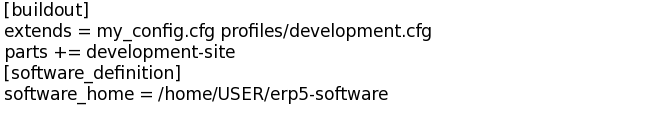
\includegraphics[scale=0.660,bb=50 50 410 120]{instancia.png}
\end{center}
\caption{Arquivo de configuração para criação da intância ERP5. Fonte: \cite{erp5_buildout}.}
\label{fig:erp5_site}
\end{figure}

\begin{figure}[ht]
\centering
\begin{center}

\includegraphics[scale=0.660,bb=0 40 410 0]{criar_instancia_erp5.png}
\end{center}
\caption{Comando para criar instância ERP5. Fonte: \cite{erp5_buildout}.}
\label{fig:run_buildout_again}
\end{figure}

Por fim, o comando apresentado na Figura \ref{fig:iniciar_zope} inicia a instância. Como padrão dos arquivos de configuração, a \textit{url} para acessá-la o ERP5 é \url{http://localhost:18080/erp5} com usuário ``zope'' e senha ``zope''.

\begin{figure}[!ht]
\centering
\begin{center}

\includegraphics[scale=0.660,bb=0 50 410 0]{rodar_instancia.png}
\end{center}
\caption{Comando para iniciar instância ERP5. Fonte: \cite{erp5_buildout}.}
\label{fig:iniciar_zope}
\end{figure}

\subsection{Configurando ERP5 para utilizar o Cloudooo}

Após a instalação de toda estrutura do ERP5, foi necessário configurar o OOOD na instância instalada. Acessando a página principal do ERP5, a criação do arquivo de configuração foi realizada pela aba esquerda da mesma página, selecionando a opção ``Preferences'', como mostra a Figura \ref{fig:erp5_click_preferences}. Quando esta opção foi selecionada, a página de preferências do ERP5 foi aberta.

\begin{figure}[!ht]
\centering
\begin{center}
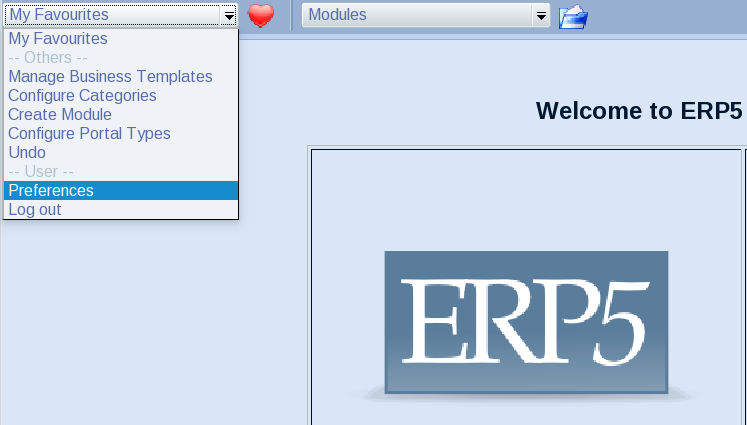
\includegraphics[scale=0.360,bb=0 0 610 290]{erp5_click_preferences.png}
\end{center}
\caption{Opção para acessar as preferências do ERP5.}
\label{fig:erp5_click_preferences}
\end{figure}

Após isto, selecionou-se a aba com nome de ``Action'' na página de prefências e a opção ``Add System Preference'', como demonstra a Figura \ref{fig:action_pref}. Um arquivo de configuração foi criado para que as configurações sejam definidas. A Figura \ref{fig:add_system_pref} apresenta o arquivo de configuração criado.

Com o arquivo de configuração criado, o próximo passo foi definir o endereço do serviço OOOD nos campos ``Conversion Server Address'' para o endereço via internet e ``Conversion Server Port'' para declarar qual porta de acesso na máquina. Por fim, foi salvo as alterações selecionando a ícone igual a um disquete no canto superior direito da página e para utiliza-la, selecionou-se a opção ``Enable Preference'' no campo ``Action''. 

\begin{figure}[!ht]
\centering
\begin{center}
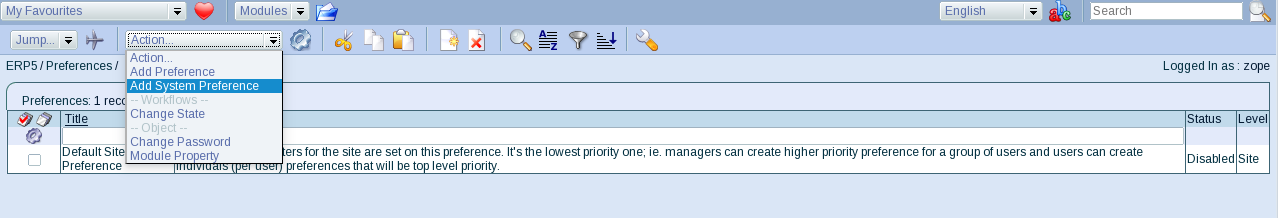
\includegraphics[scale=0.460,bb=0 0 1010 130]{action_pref.png}
\end{center}
\caption{Página de prefêrencias da instância ERP5.}
\label{fig:action_pref}
\end{figure}

\begin{figure}[!ht]
\centering
\begin{center}
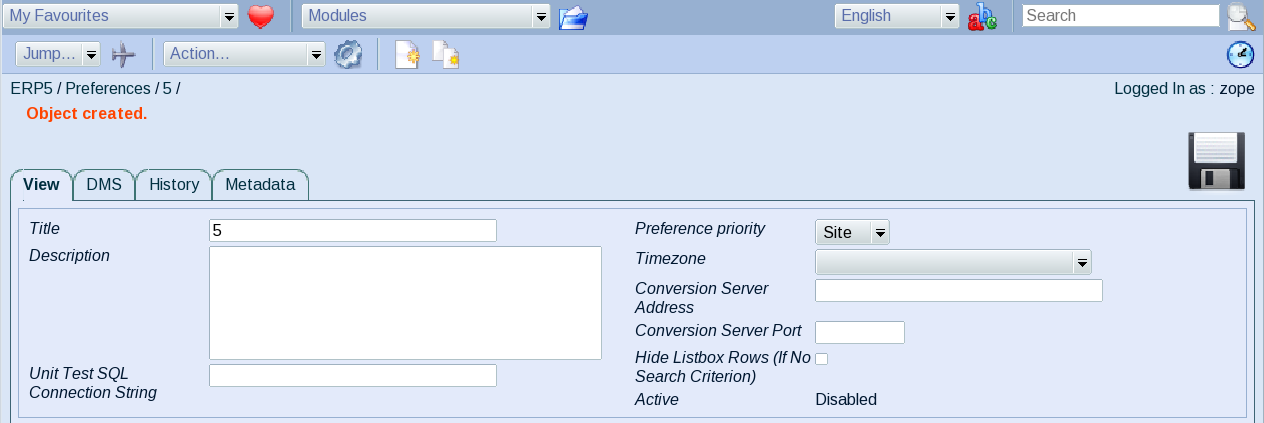
\includegraphics[scale=0.460,bb=0 0 1010 300]{add_system_pref.png}
\end{center}
\caption{Arquivo de configuração da instância.}
\label{fig:add_system_pref}
\end{figure}

\subsection{Instalação do \textit{Business Template} erp5\_dms}

Para que fosse possível inserir documentos no ERP5 foi necessário utilizar o \textit{Business Template}(BT5) erp5\_dms. Para instalação deste pacote acessou-se a principal do ERP e selecionou-se a opção ``Manage Business Templates'' no campo de nome ``My Favourites'', situado no canto esquerdo da mesma página, demonstrado na Figura \ref{fig:manage_bt5}.

\begin{figure}[!ht]
\centering
\begin{center}
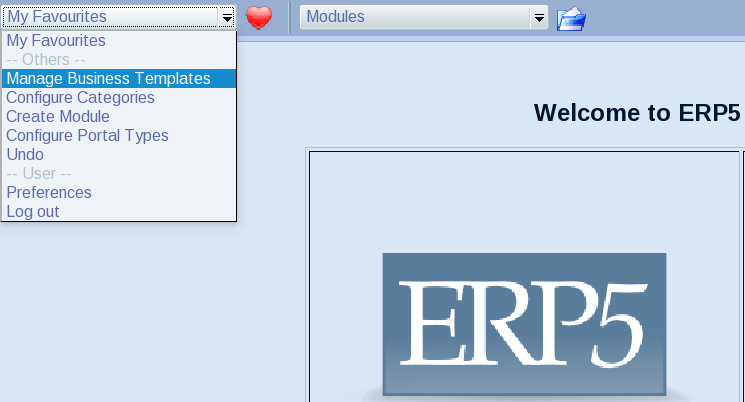
\includegraphics[scale=0.430,bb=0 45 610 257]{manage_bt5.png}
\end{center}
\caption{Opção para acessar a página de configuração dos \textit{Business Templates}.}
\label{fig:manage_bt5}
\end{figure}

Após isto, foi selecionado o botão ``Import \ Export'', indicado pela seta na Figura \ref{fig:import_export.png}, para que a página de atualização dos \textit{Business Templates} fosse aberta. No campo "Repositories" definiu-se o repositório \url{http://www.erp5.org/dists/snapshot/bt5}. A Figura \ref{fig:update_bt5.png} demonstra a página de atualização e o campo a ser preenchido.

\begin{figure}[!ht]
\centering
\begin{center}
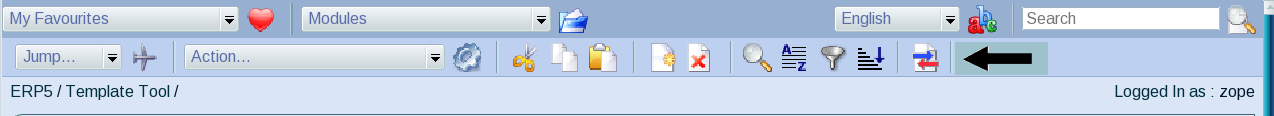
\includegraphics[scale=0.490,bb=0 30 1010 70]{import_export.png}
\end{center}
\caption{Botão para importar ou exportar \textit{Business Templates}.}
\label{fig:import_export.png}
\end{figure}

\begin{figure}[!ht]
\centering
\begin{center}
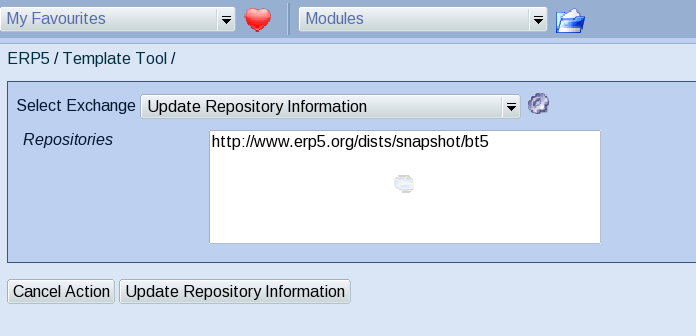
\includegraphics[scale=0.490,bb=0 30 510 210]{update_bt5.png}
\end{center}
\caption{Página para definir o endereço do repositório a ser utilizado.}
\label{fig:update_bt5.png}
\end{figure}

Definindo o repositório a ser utilizado, clicou-se em ``Update Repository Information'' para salvar a \textit{url} adicionada e, após isto, selecionou-se a opção ``Install Business Templates from Repositories'' no campo ``Select Exchange'' para que a lista de BT5 fosse exibida como demonstra a Figura \ref{fig:lista_bt5.png}.

\begin{figure}[!ht]
\centering
\begin{center}
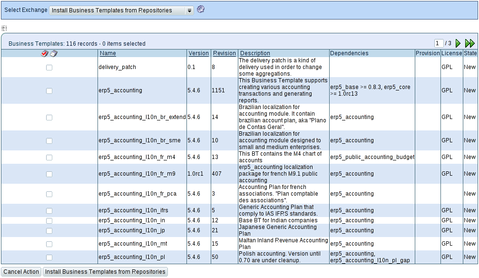
\includegraphics[scale=0.620,bb=0 30 410 190]{lista_erp5.png}
\end{center}
\caption{Lista de \textit{Business Templates} instaláveis. Fonte: \cite{erp5_bt5}.}
\label{fig:lista_bt5.png}
\end{figure}

Na página de listagem dos \textit{Business Templates}, selecionou-se os seguintes pacotes para instalação do erp5\_dms:
\begin{itemize}
 \item erp5\_base
 \item erp5\_dms;
 \item erp5\_web;
 \item erp5\_ingestion;
 \item erp5\_ingestion\_mysql\_innodb\_catalog;
\end{itemize}

Feito a seleção dos pacotes, clicou-se em ``Install Business Templates from Repositories'' no final da página e uma janela de validação de todos arquivos instaladaos foi exibida, como demonstra a Figura \ref{fig:validate_packages}. Para validar a instalação clicou-se em ``Validate Installation'' para que todos os pacotes fosse instalados.

\begin{figure}[!ht]
\centering
\begin{center}
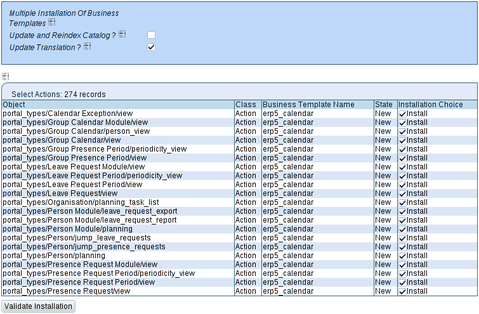
\includegraphics[scale=0.620,bb=0 30 390 210]{validate_packages.png}
\end{center}
\caption{Lista de \textit{Business Templates} instaláveis. Fonte: \cite{erp5_bt5}.}
\label{fig:validate_packages}
\end{figure}

\section{Compatibilidade entre o ERP5 e o Cloudooo}

Como o ERP5 possui muitos ambientes em produção, o custo para migrar todos estes ambientes para uma nova API seria muito grande. De tal forma, foi implementado uma interface de compatibilidade entre a aplicação Web e o ERP para redução de custo de migração para a nova API. Com isso, haverá a diminuição de falhas em ambientes de produção. Por exemplo, o metódo apresentado na Figura \ref{fig:run_convert} recebe os parâmetros da mesma forma que são enviados pelo ERP5, chama o metódo da nova API e retorna os dados como é esperado pelo ERP5.

\begin{figure}[!ht]
\centering
\begin{center}
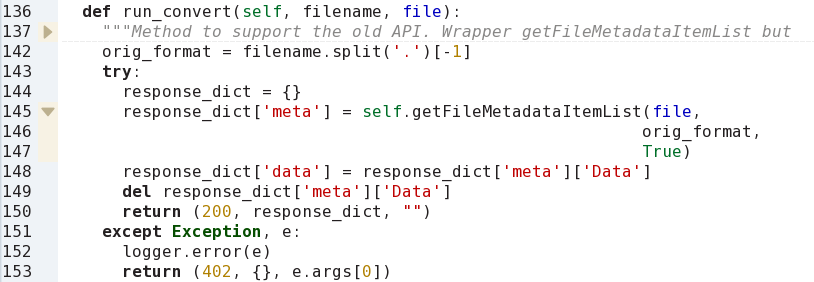
\includegraphics[scale=0.660,bb=0 0 600 190]{run_convert.png}
\end{center}
\caption{Trecho de código que representa um dos métodos de compatibilidade entre aplicações.}
\label{fig:run_convert}
\end{figure}

\section{Usando o ERP5 para converter documentos}

O OOOD é utilizado dentro do ERP5 para converter e extrair metadados de documentos. Para enviar um documento para o ERP5 clicou-se no \textit{link} ``Documents'' na página principal do ERP, como demonstra a Figura \ref{fig:erp5_click_documents}.

\begin{figure}[!ht]
\centering
\begin{center}
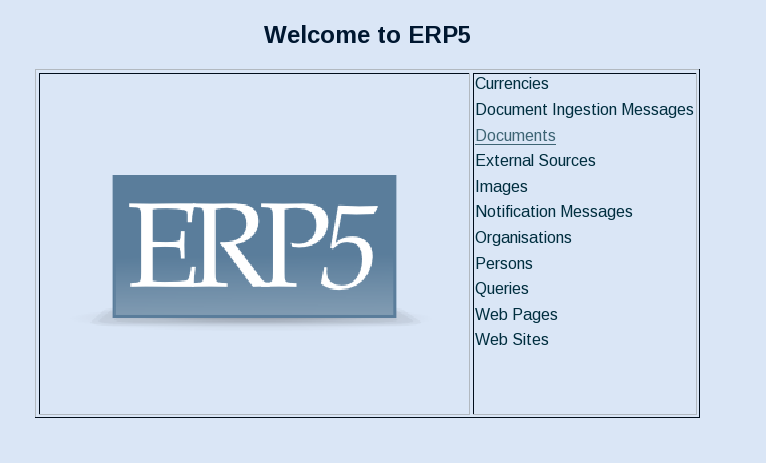
\includegraphics[scale=0.400,bb=0 40 600 310]{erp5_click_documents.png}
\end{center}
\caption{Página Principal do ERP5.}
\label{fig:erp5_click_documents}
\end{figure}

Após isto, na aba ``Action'' selecionou-se a opção ``Add Text'', demonstrado na Figura \ref{fig:add_text}. Na página seguinte foi inserido o documento e o nome para este, como mostra a Figura \ref{fig:upload_text}. Note que nesta mesma figura, quando o arquivo foi inserido e salvo, o estado deste arquivo é alterado de ``Empty'', depois para ``Converting'' e por fim ``Converted''. Isto significa que o documento foi enviado para extrair os metados e convertido para a base ODF.

\begin{figure}[!ht]
\centering
\begin{center}
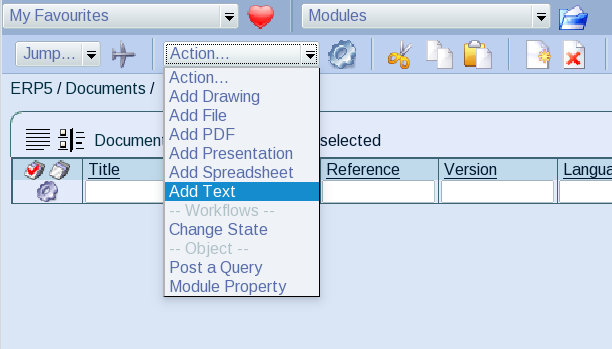
\includegraphics[scale=0.570,bb=0 30 510 240]{add_text.png}
\end{center}
\caption{Opção para criar um objeto documento no ERP5.}
\label{fig:add_text}
\end{figure}

\begin{figure}[!ht]
\centering
\begin{center}
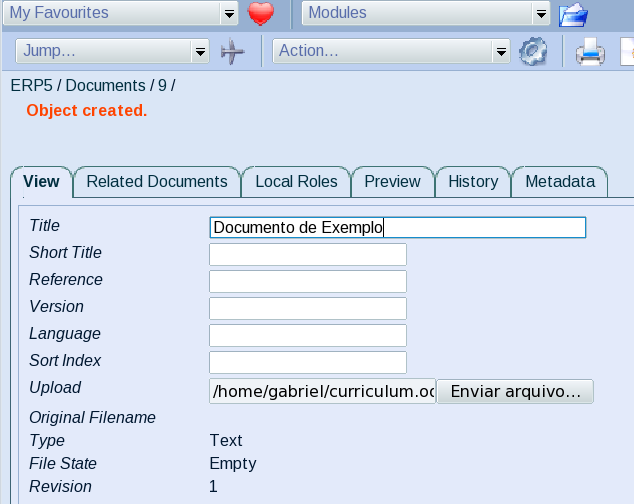
\includegraphics[scale=0.570,bb=0 30 510 340]{upload_text.png}
\end{center}
\caption{\textit{Upload} de um documento.}
\label{fig:upload_text}
\end{figure}

Para este documento ser vizualizado através do ERP5, clicou-se na aba ``Preview'', como demonstra a Figura \ref{fig:preview_erp5}. Quando a opção de vizualização foi selecionada, o documento foi convertido para o formato html para que seja possível vizualizá-lo no ERP.

\begin{figure}[!ht]
\centering
\begin{center}
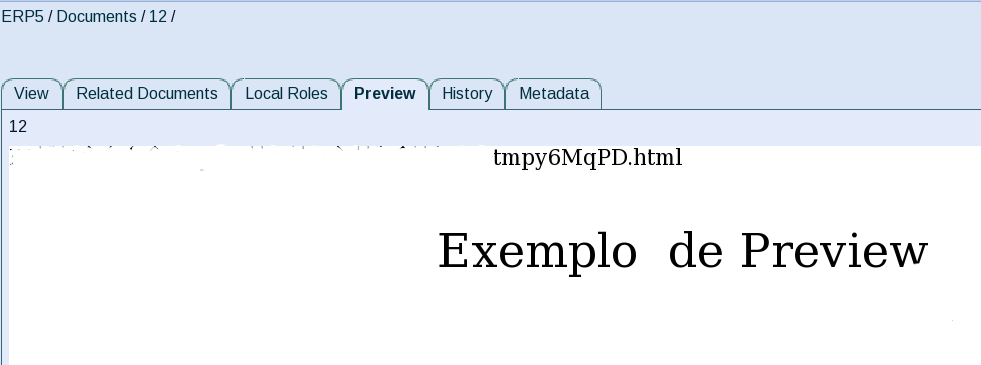
\includegraphics[scale=0.570,bb=0 30 810 240]{preview_erp5.png}
\end{center}
\caption{Pré-visualização de um documento.}
\label{fig:preview_erp5}
\end{figure}

Além disso, em documentos em formatos para apresentação é possível através da aba \textit{Preview} fazer \textit{download} do documento completo no formato pdf. Para isto, clicou-se em ``Download as PDF'' no final da página de pré-vizualização.

\section{Problemas e Decisões de Projeto}

Com o desenvolvimento e testes excessivos na aplicação, algumas decisões de projeto foram tomadas para obter resultados mais eficientes ao clientes e correção de erros graves. Nesta sessão é explicado decisões que, em alguns casos, mudaram a arquitetura do projeto.

\subsection{Vazamento de memória}

O uso excessivo da aplicação OOOD mostrou que em algumas conexões entre o UNO e o OpenOffice.org, a memória utilizada não era completamente liberada. Este aumento gradativo do uso da memória, ocasiona um erro no sistema operacional, chamado \textit{memory leak}, que ocorre quando não há mais memória livre para ser utilizada. 

Com os resultados dos testes e a análise do uso de memória, foi possível detectar que o erro está no UNO que não libera a memória corretamente quando a conexão com o OpenOffice.org termina. Além disso, foi detectado também que a memória somente é liberada corretamente quando todo o processo é finalizado, ou seja, quando o serviço é parado. Para que isso fosse resolvido foi necessário remover a biblioteca UNO da memória quando esta não estivesse sendo utilizada.

A solução para este problema foi a implementação de dois \textit{scripts} que fazem toda comunicação entre o OOOD e o OpenOffice.org. Desta forma, quando os \textit{scripts} terminarem os procedimentos, toda memória utilizada será liberada e o serviço não sofrerá alteração, caso ocorram falhas.

Estes \textit{scripts} foram implementados com objetivos diferentes, logo, as sessões abaixo explicam cada \textit{script} e seus objetivos.

\subsubsection{UnoConverter}

O \textit{script UnoConverter} foi implementado para conter as mesmas funcionalidades que o \textit{OOHandler}. Esta implementação tem como objetivo retirar a comunicação entre OOOD e o OpenOffice.org. Com isso, o \textit{OOHandler} utiliza o \textit{script UnoConverter} para se comunicar com o OpenOffice.org.

Desta forma, a memória utilizada pela comunicação entre o \textit{script UnoConverter} e o OpenOffice.org é liberada assim que o \textit{script} é finalizado.

\subsubsection{UnoMimeMapper}

Além do acesso constante para conversão de documentos, uma outra necessidade de acesso ao OpenOffice.org é a extração de filtros feito pelo \textit{MimeMapper}. Como este é um componente da aplicação OOOD, o \textit{UnoMimeMapper} é utilizado para extrair os filtros do OpenOffice.org e retorná-los para o \textit{MimeMapper}.

\subsection{Armazenamento e busca dos filtros}

A partir da extensão de um documento, como por exemplo ``doc'', é possível saber para quais formatos este documento pode ser exportado. Com o objetivo de fazer com que esta funcionalidade tenha um desempenho melhor, foram criadas três estruturas que armazenam as informações de maneiras diferentes para minimizar o tempo de busca pelos dados. As três maneiras são:

\begin{itemize}
\item Filtro por Extensão - armazena os filtros a partir da extensão do arquivo. Utilizada para selecionar o filtro adequado para exportar o documento;

\item Extensões por Tipo de documento - armazena extensões de acordo com o seu tipo. Utilizado para buscar extensões de acordo com o tipo do documento;

\item Tipo de Documento por extensão - armazena os tipos dos documentos suportados pela extensão. Com esta estrutura é possível verificar se a extensão de destino do documento suporta o mesmo tipo que a extensão do arquivo original;
\end{itemize}

Em suma, durante a importação dos filtros, os dados extraídos são organizados para eliminar qualquer processamento na hora de buscar por informações.

\subsection{Arquivos compactados}

Arquivos no formato ``html'' e ``htm'' não suportam imagens dentro do corpo do arquivo. Para que a imagem seja visualizada junto com o conteúdo em páginas Web, o caminho da imagem é inserido dentro código do documento. Como a aplicação OOOD suporta conversões de documentos, tanto o arquivo enviado ou recebido pelo o cliente em formatos ``html'' ou ``htm'', é necessário que as imagens sejam enviadas junto com o documento, caso contrário o documento gerado será inválido. Para que isto seja possível, o \textit{FileSystemDocument} suporta compactação e descompactação de arquivos.

O caso de descompactação ocorre quando o cliente envia um arquivo e este está compactado. Neste caso, todos os dados são extraídos, salvos na mesma pasta, o arquivo original é removido e o arquivo com nome \textit{index.html} é posto como documento principal.

Em contrapartida, a compactação é requisitada pelo usuário e, caso seja, o \textit{FileSystemDocument} compacta todos arquivos que estão dentro da pasta e envia para o cliente.

\section{Explicando o funcionamento do prestador de serviço com \textit{Paste}}

Para provêr os serviços do OOOD, foi utilizado a ferramenta \textit{Paste}, que é um conjunto de ferramentas para construção de aplicativos e, além disso, provê serviços que implementam a interface WSGI.

Para configurar a aplicação OOOD com o \textit{Paste}, foi definido no arquivo \textit{setup.py} da aplicação, qual metódo seria utilizado para iniciar o serviço, como demonstra a Figura \ref{fig:setup}.

Com a definição apresentada pela Figura \ref{fig:setup}, o método de nome \textit{application} será responsável por iniciar o serviço. Além disso, este mesmo método, de acordo com o WSGI, deve retornar no final de seu procedimento qual método o cliente recebe ao se conectar com o serviço.

\begin{figure}[!ht]
\centering
\begin{center}
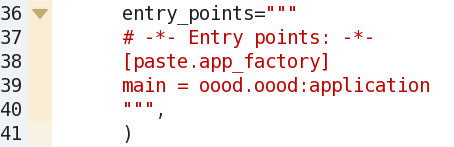
\includegraphics[scale=0.620,bb=0 30 310 100]{setup_py_paste.png}
\end{center}
\caption{Definição do metódo que irá prover o serviço.}
\label{fig:setup}
\end{figure}

\begin{figure}[!ht]
\centering
\begin{center}
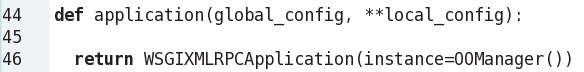
\includegraphics[scale=0.620,bb=0 30 510 60]{oood_application.png}
\end{center}
\caption{Método que inicia a aplicação e retorno do objeto que o cliente recebe quando se conecta.}
\label{fig:application}
\end{figure}

Por fim, para iniciar uma aplicação utilizando a ferramenta \textit{Paste}, esta última necessita de um arquivo de configuração que possui informações como, o pacote do \textit{Paste} a ser utilizado e a porta que o servidor deve ser iniciado. A Figura \ref{fig:oood_conf} demonstra um trecho do arquivo de configuração para iniciar a aplicação OOOD e a Figura \ref{fig:start_paste} demonstra como a aplicação é iniciada utilizando esta aplicação.

\begin{figure}[!ht]
\centering
\begin{center}
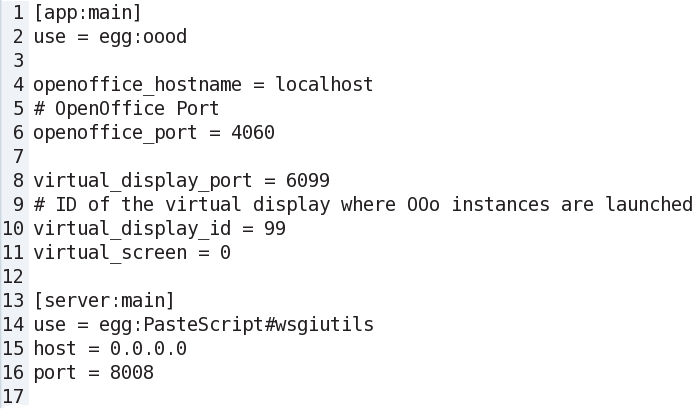
\includegraphics[scale=0.520,bb=0 30 510 280]{oood_conf.png}
\end{center}
\caption{Amostra do arquivo de configuração.}
\label{fig:oood_conf}
\end{figure}

\begin{figure}[!ht]
\centering
\begin{center}
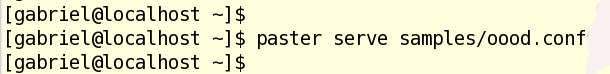
\includegraphics[scale=0.570,bb=0 30 510 0]{start_paste.png}
\end{center}
\caption{Iniciando a aplicação OOOD com \textit{Paste}.}
\label{fig:start_paste}
\end{figure}

\section{Comparando a \textit{perfomance} entre a Cloudooo e o OOOD}

Para comparar melhor o desenvolvimento da nova aplicação, foram desenvolvidos \textit{scripts} que submetiam documentos tanto para nova aplicação quanto para a antiga. Nestes scripts, foram registrados o tempo de conversão de cada documento e o tempo total de todas as conversões.

Para realização destes testes foram selecionados 3699 documentos no formato odt, sendo alguns destes inválidos e outros em formatos desconhecidos. Além disso, para realização destes testes foi definido que o formato destino dos documentos fosse o pdf, pois este formato é o mais utilizado pelo ERP5 para exportar documentos.

Com o resultado dos testes, notou-se que a conversão do primeiro documento é mais rápida no OOOD. Mas, com o uso excessivo das aplicações e com os erros gerados, o Cloudooo se manteve estável enquanto o OOOD apresentou-se instável em relação ao tempo de conversão. Os erros apresentados pelo Cloudooo foram 12 de arquivos inválidos, enquanto a aplicação antiga apresentou 531 erros.

Apesar do Cloudooo individualmente ser mais lento para arquivos individuais, o tempo gasto para conversão de todos foi de 10 horas. Enquanto a aplicação antiga gastou 11 horas para finalizar as conversões.

\section{Resultados obtidos}

No estudo de caso foi apresentado a utilização da aplicação OOOD junto com a ferramenta \textit{Paste}, que provê o serviço. Além disso, foi  instalado e configurado o ERP5 e o \textit{Business Templates} para conversão e extração de metadados de documentos utilizando o OOOD.

Vale ressaltar que, a ferramenta que provê o serviço utilizada neste estudo de caso, pode ser substituída por qualquer outra ferramenta que forneça serviços que utilizem o padrão WSGI. Isto demonstra que o serviço pode ser modificado de acordo com a necessidade e demanda dos clientes.

Além disso, foram apresentados dados comprovando que com a utilização de uma arquitetura mais atual e flexível, trouxeram resultados satisfátorios.